% Document class, paper size, base font size
\documentclass[a4paper, 10pt]{article}

% Farben
\usepackage[dvipsnames]{xcolor}

% Farben für Code Listings Style
\definecolor{codegreen}{rgb}{0,0.6,0}
\definecolor{codegray}{rgb}{0.1,0.1,0.1}
\definecolor{codepurple}{rgb}{0.58,0,0.82}
\definecolor{backcolour}{rgb}{0.95,0.95,0.95}

% code listings
\usepackage{listings}

% Style für Code Listings
\lstdefinestyle{mystyle}{
    backgroundcolor=\color{backcolour},   
    commentstyle=\color{codegreen},
    keywordstyle=\bfseries\color{magenta},
    numberstyle=\tiny\color{codegray},
    stringstyle=\color{codepurple},
    basicstyle=\ttfamily\footnotesize,
    breakatwhitespace=false,         
    breaklines=true,                 
    captionpos=b,                    
    keepspaces=true,                 
    numbers=left,                    
    numbersep=5pt,                  
    showspaces=false,                
    showstringspaces=false,
    showtabs=false,                  
    tabsize=2,
    belowskip=-2mm,
    aboveskip=-3mm
}

\lstset{style=mystyle}

% Encoding
\usepackage[utf8]{inputenc}
\usepackage[T1]{fontenc}

% Title, authors and date
\title{Exercise 1: Probeklausur Objektorientierte Programmierung Grundlagen}
\author{
    Kendra Birringer (1229372)\\
    Nader Cacace (1208115)\\
    Steffen Hanzlik (1207417)\\
    Marco Peluso (1228849)\\
    Svetozar Stojanovic (1262287)\\
    \\
    Frankfurt University of Applied Sciences
}
\date{November 1st, 2019}

% Prevent indentation of beginning of paragraphs
\setlength{\parindent}{0em}

% Space between paragraphs
\parskip 0.5em

% include PDFs
\usepackage{pdfpages}

% captions
\usepackage[font={small, it}]{caption}
\captionsetup{justification=raggedright, singlelinecheck=false}

% keep figures in place
\usepackage{float}

\begin{document}
\maketitle

\newpage
\tableofcontents
\listoffigures

\newpage
\section{Exercise 3}
\subsection{EBook Headerfile}
\begin{figure}[ht]
\begin{lstlisting}[language=c++]
#ifndef _EBOOK_H_
#define _EBOOK_H_

#include <string>
#include <iostream>

using namespace std;

class EBook {
private:
  string title, content;
public:
  EBook();
  EBook(string title, string content);
  void setTitle(string title);
  string getTitle() const;
  void setContent(string content);
  string getContent() const;
  void print() const;
  friend ostream &operator<<(ostream &output, const EBook &book);
};

#endif
\end{lstlisting}
\caption{Header of EBook Program}
\end{figure}
In the header file the declaration of the private and the public members of the EBook class takes place.

The private members are two Strings named 'title' and 'content'.
The public members of the class EBook are the default constructor and an overloaded constructor with the parameters title and content.

Then we also declared the public 'getter' and 'setter' methods. Furthermore we need a print method and we must overload the \&operator$<<$ method.

\newpage
\subsection{Implementation of the EBook class}
\begin{figure}[H]
\begin{lstlisting}[language=c++]
#include "eBook.h"
#include <iostream>

using namespace std;

EBook::EBook() : title(""), content("") {};

EBook::EBook(string title, string content) : title(title), content(content) {};

void EBook::setTitle(string title) {
  if (title != "") {
    this->title = title;
  } else {
    cout << "Title not set!" << endl;
  }
}
string EBook::getTitle() const {
  return this->title;
}
void EBook::setContent(string content) {
  if (content != "") {
    this->content = content;
  } else {
    cout << "Content not set!" << endl;
  }
}
string EBook::getContent() const {
  return this->content;
}

void EBook::print() const {
  cout << "Title: " << this->title << '\n';
  cout << "Content: " << this->content << '\n';
}

ostream & operator<<(ostream &output, const EBook &book) {
  book.print();
  return output;
\end{lstlisting}
\caption{Implementation of EBook class}
\end{figure}
In the Ebook.cpp file we implemented the declared methods of Ebook.h.
First we implemented the standard constructor initializing the member variables 'title' and 'content' using an initializer list.

Furthermore we implemented an overloaded constructor of Bbook with the arguments 'title' and 'content' and initialized the 'title' and 'content' with the passed arguments 'title' and 'content'.

Then we implemented the 'getter' and 'setter' methods.
Also we implemented the 'print' method. This method is for printing the 'title' and the 'content' and we overloaded the \&operater$<<$ method.

\subsection{Main class}
\begin{figure}[H]
\begin{lstlisting}[language=c++]
#include <iostream>
#include "eBook.h"

int main() {
  EBook book("Brown Fox", "The quick brown fox jumps over the lazy dog.");
  std::cout << book;

  return 0;
}
\end{lstlisting}
\caption{Main class of Ebook program}
\end{figure}
The main method executes the EBook class.

\newpage
\section{Exercise 4}
\subsection{Form Headerfile}
\begin{figure}[H]
\begin{lstlisting}[language=c++]
#ifndef _FORM_H_
#define _FORM_H_

#include "Box.h"

class Form {
private:
  double xCenter, yCenter;
protected:
  Box box;
public:
  Form();
  void move(double dX, double dY);
  Box &getBoxRef();
};
#endif
\end{lstlisting}
\caption{Header of Form class}
\end{figure}
This header file declares a class 'Form', which is the base class for classes 'Circle' and 'Rectangle'. The private members of this class are two double variables 'xCenter' and 'yCenter', which store coordinates for the center of the form.
The protected member is a Box type object called 'box'. Because of this, every class that derives from 'Form' class has its own 'box' member and it cannot be accessed directly outside of this class.

As public members we have a default constructor called 'Form()', a 'move' method that changes the coordinates of the form depending on the passed parameters 'dX' and 'dY', and a method called 'getBoxRef()' that returns a reference to the 'Box' type object in this class.

\subsection{Implementation of Form class}
\begin{figure}[H]
\begin{lstlisting}[language=c++]
#include "Form.h"

Form::Form() : xCenter(0.0), yCenter(0.0) {

}

void Form::move(double dX, double dY) {
  this->xCenter += dX;
  this->yCenter += dY;
}

Box & Form::getBoxRef() {
  return box;
}
\end{lstlisting}
\caption{Form class Implementation}
\end{figure}
Here we implemented the methods which we declared in the related header file.

\subsection{Box Headerfile}
\begin{figure}[H]
\begin{lstlisting}[language=c++]
#ifndef _BOX_H_
#define _BOX_H_

class Box {
private:
  double xMin, xMax, yMin, yMax;
public:

  Box();
  double getXMin() const;
  double getXMax() const;
  double getYMin() const;
  double getYMax() const;
  void setXMax(double val);
  void setXMin(double val);
  void setYMin(double val);
  void setYMax(double val);
  friend Box operator+(Box left, Box right);
  void print() const;
};
#endif
\end{lstlisting}
\caption{Header of Box class}
\end{figure}
In the header file the declaration of the private and the public members of the Box class takes place.

The 'Box' class is the representation of the bounding for each form. It is included as an object in 'Form', 'Circle' and 'Rectangle' classes.

The private members of this class are variables 'xMin', 'xMax', 'yMin' and 'yMax'.

The public members are typical getter und setter conventional methods for this class, also an overloaded constructor 'Box()' that zero-initializes the private members, a 'print' method to display the bounding box values for this class, and an overloaded '+' operator declared as a friend function. It is important to declare the overloaded operator as a friend function because we want to directly access private data members.

Also, this overloaded operator's purpose is to create a new bounding box only if the two 'Box' type objects passed as arguments.

\subsection{Implementation of the Box class}
\begin{figure}[H]
\begin{lstlisting}[language=c++]
#include "Box.h"
#include <iostream>
#include <algorithm>

using namespace std;

Box::Box() : xMin(0.0), xMax(0.0), yMin(0.0), yMax(0.0) {

}

double Box::getXMin() const {
  return xMin;
}

void Box::setXMax(double val) {
  this->xMax = val;
}

double Box::getXMax() const {
  return xMax;
}

void Box::setXMin(double val) {
  this->xMin = val;
}

double Box::getYMin() const {
  return yMin;
}

void Box::setYMin(double val) {
	this->yMin = val;
}

double Box::getYMax() const {
	return yMax;
}

void Box::setYMax(double val) {
	this->yMax = val;
}

void Box::print() const {
	cout << "xMax: " << xMax << endl;
	cout << "xMin: " << xMin << endl;
	cout << "yMax: " << yMax << endl;
	cout << "yMin: " << yMin << endl;
}
\end{lstlisting}
\caption{Box class Implementation – Part 1}
\end{figure}

\begin{figure}[H]
\begin{lstlisting}[language=c++]
Box operator+(Box left, Box right) {
	Box newLeft, newRight;
	if (left.getXMax() > right.getXMax()) {
		newLeft = right;
		newRight = left;
	} else {
		newLeft = left;
		newRight = right;
	}

	Box result;

	//check if the boxes collide
	if (right.getXMin() < left.getXMax() && right.getYMin() < left.getYMax()) {
		result.setXMin(min(newLeft.getXMin(), newRight.getXMin()));
		result.setXMax(max(newLeft.getXMax(), newRight.getXMax()));
		result.setYMin(min(newLeft.getYMin(), newRight.getYMin()));
		result.setYMax(max(newLeft.getYMax(), newRight.getYMax()));
		return result;
	} else {
		cout << "The boxes of these two objects don't collide." << '\n';
	}
}
\end{lstlisting}
\caption{Box class Implementation - Part 2}
\end{figure}
In the Box class we implemented getter and setter Methods. Also we implemented the print method to show the Min and Max coordinate. Then we overload the  operator$+$ method.

Here are all methods from the header file implemented.

The overloaded operator '+' checks if the bounding boxes collide and if so, displays a message to the user.

\subsection{Circle Headerfile}
\begin{figure}[H]
\begin{lstlisting}[language=c++]
#ifndef _CIRCLE_H_
#define _CIRCLE_H_

#include "Form.h"

class Circle : public Form
{
private:
	double radius;
public:
	Circle();
	Circle(double rad);
	void move(double dX, double dY);
	void initBox();
private:
	void moveBox(double dX = 0, double dY = 0);
};
#endif
\end{lstlisting}
\caption{Header of Circle class}
\end{figure}
In the header file of the Circle class we declare the private and public members. One of the private members is a double type variable named 'radius'. The other private member is a method named 'moveBox' with the Arguments 'dX' and 'dY'. The public members are the standard and a overloaded constructor with the parameter 'rad' which is a double type variable. The other public members are the 'move' method with the two arguments 'dX' and 'dY' and a 'initBox' method.

Before declaring the 'Circle' class we must first include the base class 'Form' (see the line number 4).

This header file declares a 'Circle' class, derived from the 'Form' class.
In the private section we have a double variable 'radius' and a function 'moveBox'. Variable 'radius' stores the radius of the circle and the function 'moveBox' changes the position of the bounding box for this form.

The public methods are two overloaded constructors 'Circle()' and 'Circle(double rad)', a 'move' method that changes the position of the circle, and a method 'initBox' that initializes the bounding box.

\subsection{Implementation of Circle class}\begin{figure}[H]
\begin{lstlisting}[language=c++]
#include "Circle.h"

Circle::Circle() : radius(0.0) {
	Form();
	this->box.setXMax(0.0);
	this->box.setXMin(0.0);
	this->box.setYMax(0.0);
	this->box.setYMin(0.0);
}

Circle::Circle(double rad) : radius(rad) {

}

void Circle::initBox() {
	this->box.setXMax(this->radius);
	this->box.setXMin(-this->radius);
	this->box.setYMax(this->radius);
	this->box.setYMin(-this->radius);
}

void Circle::move(double dX, double dY) {
	Form::move(dX, dY);
	moveBox(dX, dY);
}

void Circle::moveBox(double dX, double dY) {
	this->box.setXMax(box.getXMax() + dX);
	this->box.setXMin(box.getXMin() + dX);
	this->box.setYMax(box.getYMax() + dY);
	this->box.setYMin(box.getYMin() + dY);
}

\end{lstlisting}
\caption{Circle class Implementation}
\end{figure}
In the Circle class we implemented the default constructor and the overloaded constructor aswell. Furthermore we set all coordinates for the Box that surround the circle object in the initBox method. We also wrote a move method to move the circle and a moveBox method that gets called from the move method to shift the Box to the same place.

The first overloaded constructor 'Circle()' just initializes the 'radius' variable with zero.
The second overloaded constructor 'Circle(double rad)' initializes the 'radius' variable with the value of the parameter 'rad'.

Method 'initBox' of the Circle class initializes the values of the 'box' object of the 'Circle' class.

The overloaded method 'move' calls the 'move' function of its base class 'Form' and the private method 'moveBox' that changes the values of the bounding box. This makes the bbox follow the circle.

\subsection{Rectangle Headerfile}
\begin{figure}[H]
\begin{lstlisting}[language=c++]
#ifndef _RECTANGLE_H_
#define _RECTANGLE_H_

#include "Form.h"

class Rectangle: public Form {
private:
	double width, height;

public:
	Rectangle();
	Rectangle(double h, double w);
	//MOVE FOR RECT
	void move(double dX, double dY);
	void initBox();
private:
	void moveBox(double dX = 0, double dY = 0);
};
#endif
\end{lstlisting}
\caption{Header of Rectangle class}
\end{figure}
Before declaring the 'Rectangle' class we must first include the base class 'Form' (see the line number 4). Then, on the line 6 we start declaring the 'Rectangle' class that derives from 'Form'.

The private methods are two double type variables 'width' and 'height' of a rectangle. In the private section we also have a function called 'moveBox' that changes the position of the bounding box for this rectangle. Since we don't need this function outside of class, we placed this function in the private section of this class.

The public methods are an overloaded default constructor, a second overloaded constructor that initializes the private variables 'width' and 'height', an overloaded method called 'move' (overloads the 'move' method in the Form class), and a method 'initBox' that initializes the 'Box' type object for this class.

\subsection{Implementation of Rectangle class}
\begin{figure}[H]
\begin{lstlisting}[language=c++]
#include "Rectangle.h"

Rectangle::Rectangle() : width(0.0), height(0.0) {

}

Rectangle::Rectangle(double h, double w) : width(w), height(h) {

}

void Rectangle::move(double dX, double dY)
{
	Form::move(dX, dY);
	moveBox(dX, dY);
}

void Rectangle::moveBox(double dX, double dY) {
	this->box.setXMax(box.getXMax()+dX);
	this->box.setXMin(box.getXMin()+dX);
	this->box.setYMax(box.getYMax()+dY);
	this->box.setYMin(box.getYMin()+dY);
}

void Rectangle::initBox() {
	this->box.setXMax(width / 2);
	this->box.setXMin(-width / 2);
	this->box.setYMax(height / 2);
	this->box.setYMin(-height / 2);
}
\end{lstlisting}
\caption{Rectangle class Implementation}
\end{figure}
The first overloaded constructor 'Rectangle()' zero-initializes the width and height of the rectangle and all variables of the 'Box' type object. The second constructor 'Rectangle(double h, double w)' takes the parameters and initializes the variables 'height' and 'width'.

The method 'initBox' takes into account that the bounding box for the rectangle is different from any other form and it initializes the variables 'xMin', 'xMax', 'yMin' and 'yMax' of the 'box' object in this class.

The overloaded method 'move' calls the 'move' function of the 'Form' class and changes the position of the rectangle according to the two parameters 'dX' and 'dY'. This method also calls the private 'moveBox' method to update the values of the 'box' object. This makes the bounding box follow the rectangle and it updates the bounding box automatically.

\subsection{Implementation of the Main Class}
\begin{figure}[H]
\begin{lstlisting}[language=c++]
#include <iostream>
#include <string>
#include "Circle.h"
#include "Rectangle.h"

using namespace std;

//checks if the user typed 'circle', returns bool
bool inputIsCircle(string);

//checks if the user typed 'rectangle', returns bool
bool inputIsRect(string);

//asks for needed values and calls circle constructor
Circle* circleCreator(bool isTrue);

//asks for needed values and calls rectangle constructor
Rectangle* rectCreator(bool isTrue);
Box addBoxes(Circle* c1, Circle* c2, Rectangle* r1, Rectangle* r2);

int main() {

	//arguments for move(...) function
	double movX, movY;

	string prompt = "";

	std::cout << "_______________________________________" << endl;

	Circle *circle1 = NULL;
	Rectangle *rect1 = NULL;

	cout << "Enter first form (rectangle or circle): ";
	cin >> prompt;

	if (inputIsCircle(prompt)) {
		circle1 = circleCreator(inputIsCircle(prompt));
		circle1->getBoxRef().print();

		cout << "Move Circle in X direction for: ";
		cin >> movX;
		cout << "Move Circle in Y direction for: ";
		cin >> movY;

		circle1->move(movX, movY);
		cout << "After Move is called: " << endl;
		circle1->getBoxRef().print();
	} else if (inputIsRect(prompt))	{
		rect1 = rectCreator(inputIsRect(prompt));
		rect1->getBoxRef().print();

		cout << "Move Rectangle in X direction for: ";
		cin >> movX;
		cout << "Move Rectangle in Y direction for: ";
		cin >> movY;

		rect1->move(movX, movY);
		cout << "After Move is called: " << endl;
		rect1->getBoxRef().print();
	}

	Circle *circle2 = NULL;
	Rectangle *rect2 = NULL;
	cout << "Enter second form (rectangle or circle): ";
	cin >> prompt;
\end{lstlisting}
\caption{Main class Implementation – Part 1}
\end{figure}

\begin{figure}[H]
\begin{lstlisting}[language=c++]
	if (inputIsCircle(prompt)) {
		circle2 = circleCreator(inputIsCircle(prompt));
		circle2->getBoxRef().print();

		cout << "Move Circle in X direction for: ";
		cin >> movX;
		cout << "Move Circle in Y direction for: ";
		cin >> movY;

		circle2->move(movX, movY);
		cout << "After Move is called: " << endl;
		circle2->getBoxRef().print();
	} else if (inputIsRect(prompt)) {
		rect2 = rectCreator(inputIsRect(prompt));
		rect2->getBoxRef().print();

		cout << "Move Rectangle in X direction for: ";
		cin >> movX;
		cout << "Move Rectangle in Y direction for: ";
		cin >> movY;

		rect2->move(movX, movY);
		cout << "After Move is called: " << endl;
		rect2->getBoxRef().print();
	}

	//ADD BOUNDING BOXES AND PRODUCE NEW ONE AS SUM
	Box boundingBox;

	cout << "Bounding Box: " << endl;
	boundingBox = addBoxes(circle1, circle2, rect1, rect2);
	if (!(boundingBox.getXMax() == 0.0 && boundingBox.getXMin() == 0.0 && boundingBox.getYMin() == 0.0 && boundingBox.getYMax() == 0.0)) {
		boundingBox.print();
	}

	cout << "_______________________________________" << endl;

	delete circle1, rect1, circle2, rect2;

	return 0;
}

Box addBoxes(Circle* c1, Circle* c2, Rectangle* r1, Rectangle* r2) {

	Box result;
	if (c1 == NULL && c2 == NULL) {
		result = r1->getBoxRef() + r2->getBoxRef();
		return result;
	} else if (c1 == NULL && r2 == NULL) {
		result = r1->getBoxRef()+ c2->getBoxRef();
		return result;
	} else if (r1 == NULL && c2 == NULL) {
		result = c1->getBoxRef()+ r2->getBoxRef();
		return result;
	} else if (r1 == NULL && r2 == NULL) {
		result = c1->getBoxRef() + c2->getBoxRef();
		return result;
	}
	return result;
}
\end{lstlisting}
\caption{Main class Implementation – Part 2}
\end{figure}

\begin{figure}[H]
\begin{lstlisting}[language=c++]
bool inputIsCircle(string prompt) {
	string circle = "circle";
	bool result = false;
	if (prompt.compare(circle) == 0) {
		result = true;
	} else {
		return result;
	}
	return result;
}

bool inputIsRect(string prompt) {
	string rect = "rectangle";
	bool result = false;
	if (prompt.compare(rect) == 0) {
		result = true;
	} else {
		return result;
	}
	return result;
}
Circle* circleCreator(bool isTrue) {
	if (isTrue) {
		double rad;

		cout << "Enter radius: ";
		cin >> rad;
		Circle *circle = new Circle(rad);
		circle->initBox();
		return circle;
	} else {
		return NULL;
	}
}
Rectangle* rectCreator(bool isTrue) {
	if (isTrue) {
		double h, w;
		cout << "Enter height: ";
		cin >> h;
		cout << "Enter width: ";
		cin >> w;
		Rectangle *rect = new Rectangle(h, w);
		rect->initBox();
		return rect;
	} else {
		return NULL;
	}
}
\end{lstlisting}
\caption{Main class Implementation – Part 3}
\end{figure}
Now, in the main function we implement all these functions. First, we included the 'iostream' directory (line 1) and the 'string' directory from the standard library (line 2).

We also need the 'Circle' and 'Rectangle' class so we included it (lines 3 and 4). To make our lives more convenient we used the using-directive for the 'std' namespace (line 6).

On the lines 9, 12, 15, 18 and 19 we declare prototype functions that all have a different purpose. These are discussed briefly bellow.

On the line 21 we start with the 'main' function. First, we declare two double type variables 'movX' and 'movY' that will be initialized depending on the user input and, later, used as arguments for the 'move' function of each form.

The declared string 'prompt' on the line 26 is used for deciding which form to create (either a circle or a rectangle).

Lines 30 and 31 declare and initialize with NULL a circle and a rectangle object.

Depending on the user input (either 'circle' or 'rectangle') only one form of these two types will be initialized (i.e. 'circle1/2' or 'rect1/2'). The creation is implemented in the 'circleCreator' and 'rectCreator' functions. The values of the bounding box are also displayed through the use of the 'print' method of the 'Box' class.

The user will be also asked to move the form in the X and Y direction. The input is stored in the 'movX' and 'movY' variables respectively and then passed to the 'move' function.
After calling the 'move' function, the 'print' method of the 'Box' class is used again to display the variables of the bounding box for this form.

The whole process repeats for the second form.

Then, on the line 93, we declare a new 'Box' type object called 'boundingBox'. This object is used to add the bboxes of the created forms. This is achieved through the use of 'addBoxes' function, a function that finds suitable values for the new, larger bounding box. Keep in mind that if the bounding boxes of the two created forms don't collide, then we don't need to find a new bounding box since they should stay separated from each other.
On the line 103 we deallocate the memory used by 'Circle' and 'Rectangle' objects.

\newpage
\section{Learning Material}
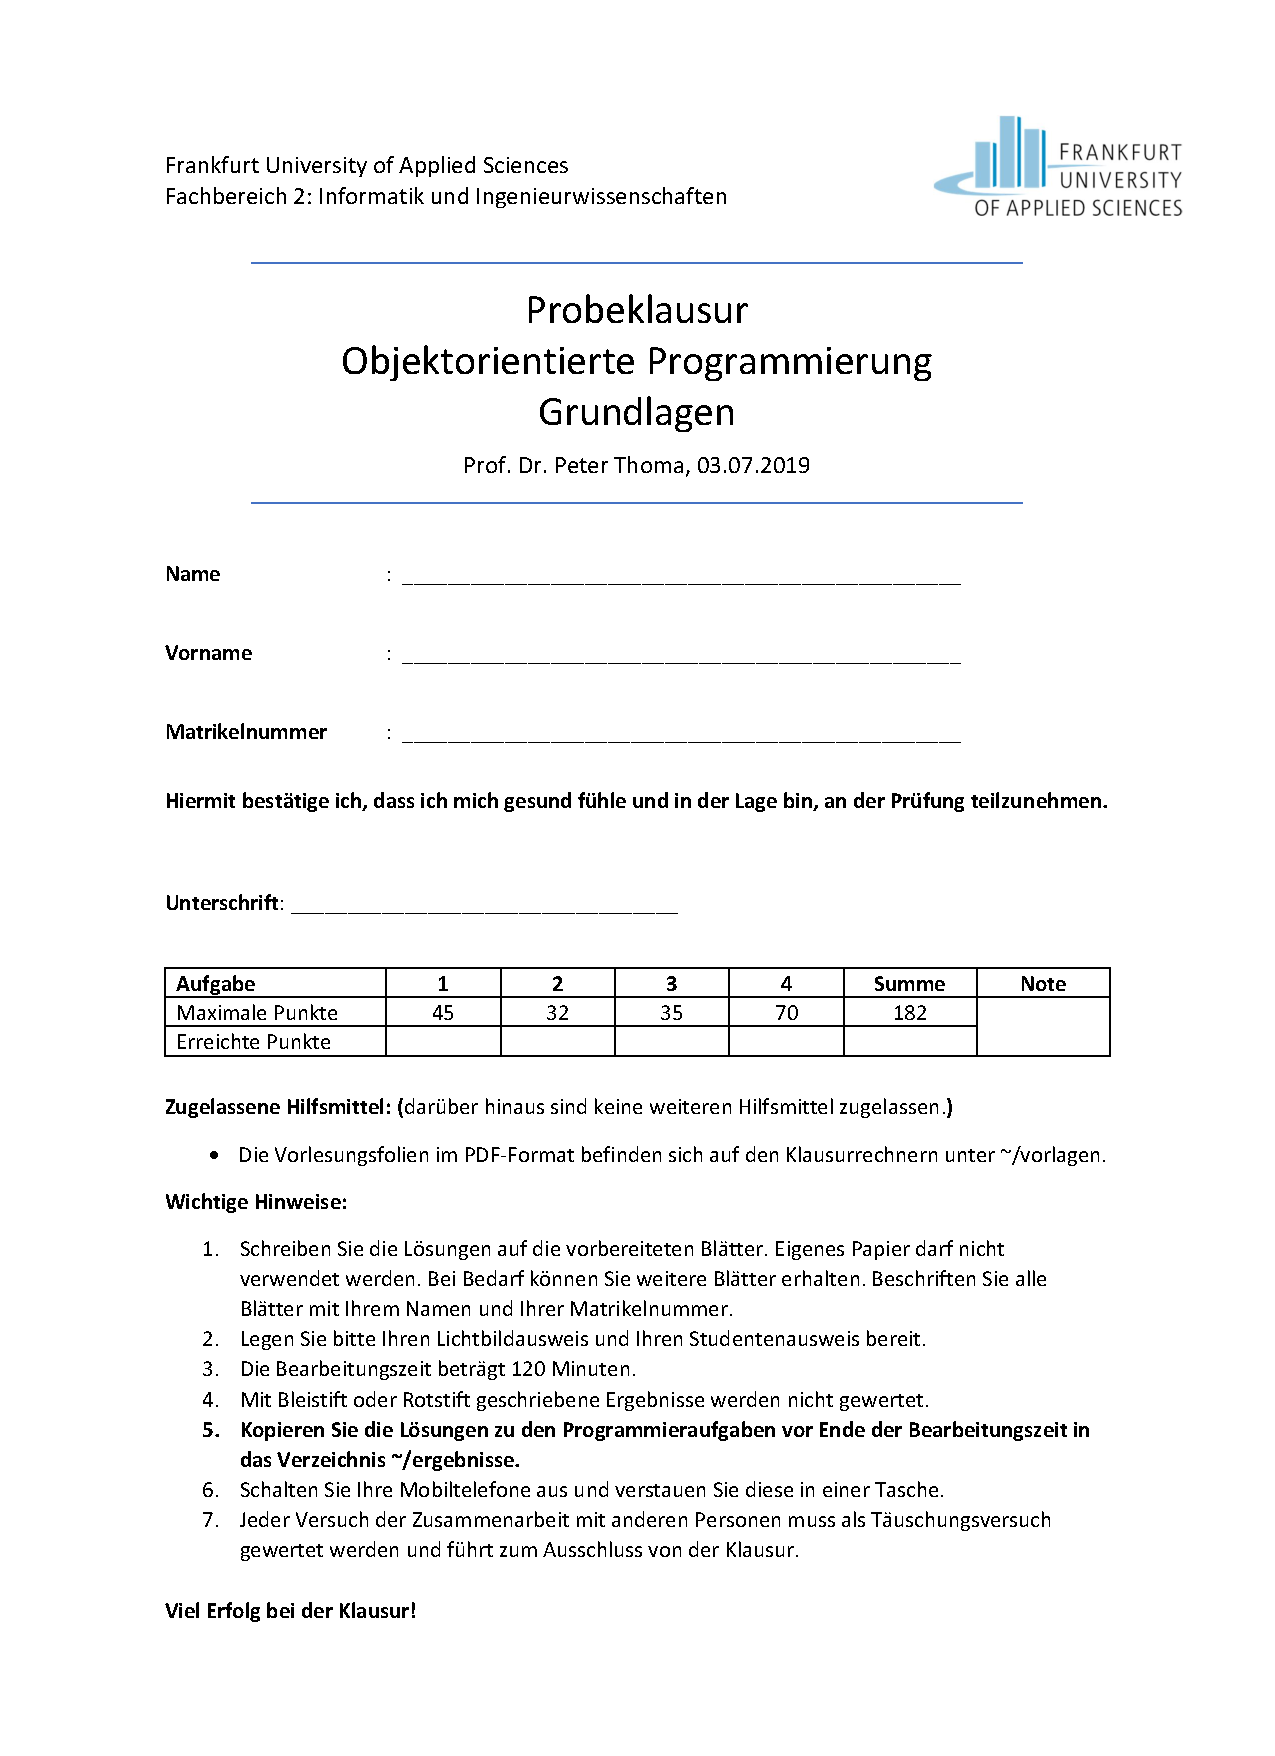
\includepdf[pages=-]{exam-solution-complete.pdf}


\end{document}